\documentclass[../00_main.tex]{subfiles}

\begin{document}

\section{Class 13.10.2020}

\subsection{Varying Annuities}

\begin{itemize}
    \item general type of a varying annuity
\begin{center}
    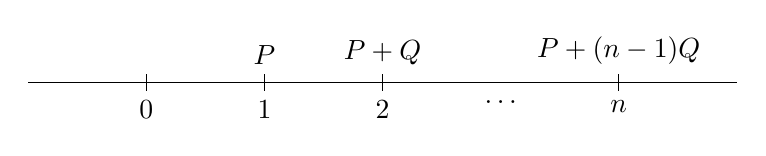
\begin{tikzpicture}
        \def\f{1.5}
        \draw (0,0) -- (\f*6,0);
        \foreach \x in {\f*1,\f*2,\f*3,\f*5}
          \draw (\x cm,3pt) -- (\x cm,-3pt);
        \draw (\f*1,0) node[below=3pt, align=center] {$0$}
            node[above=3pt] {$ $};
        \draw (\f*2,0) node[below=3pt, align=center] {$1$}
            node[above=3pt] {$P$};
        \draw (\f*3,0) node[below=3pt, align=center] {$2$}
            node[above=3pt] {$P+Q$};
        \draw (\f*4,0) node[below=3pt, align=center] {$\dots$}
            node[above=3pt] {$ $};
        \draw (\f*5,0) node[below=3pt, align=center] {$n$}
            node[above=3pt] {$P+(n-1)Q$};
    \end{tikzpicture}
\end{center}
\item we can find the value 1 year before the first payment with
    \begin{equation}\nonumber
        A = P\ax{\angln} + Q \left[ \frac{\ax{\angln} - nv^n}{i} \right]
    \end{equation}
\item the accumulated value of these payments is
    \begin{equation}\nonumber
        A(1+i)^n = P\sx{\angln} + Q \left[ \frac{\sx{\angln} - n}{i} \right]
    \end{equation}
\end{itemize}

\subsubsection{Increasing Annuity}
\begin{itemize}
    \item here $P=Q=1$
    \item the present value for this annuity is 
    \begin{equation}\nonumber
        (Ia)_{\angln} = \frac{\ax**{\angln} - nv^n}{i}
    \end{equation}
    \item the accumulated value for this annuity is 
    \begin{equation}\nonumber
        (Is)_{\angln} = \frac{\sx**{\angln} - n}{i}
    \end{equation}
\end{itemize}

\subsubsection{Decreasing Annuity}
\begin{itemize}
    \item here $P=1$ and $Q=-1$
    \item the present value for this annuity is 
    \begin{equation}\nonumber
        (Da)_{\angln} = \frac{n - \ax{\angln}}{i}
    \end{equation}
    \item the accumulated value for this annuity is 
    \begin{equation}\nonumber
        (Ds)_{\angln} = \frac{n(1+i)^n - \sx{\angln}}{i}
    \end{equation}
\end{itemize}

\subsubsection{Geometric Annuity}
\begin{itemize}
    \item here $Q$ changes in a geometric way, by $c$
    \item then the sum of this annuity can be found with
    \begin{equation}\nonumber
        \begin{gathered}
        r = \frac{1+i}{c}\\
        S_n = Q(c)^{n-1} \left[\frac{1-r^n}{1-r} \right]
        \end{gathered}
    \end{equation}
    \item to find the present value 
    \begin{equation}\nonumber
        \begin{gathered}
        r = \frac{1+i}{c}\\
        P_n = Q(c) \left[\frac{1-r^n}{1-r} \right]
        \end{gathered}
    \end{equation}
\end{itemize}

\end{document}
